% Two slides: properties of the delta network, and how the extracted graph is cleaned.
% To use in the main deck: copy the two frames below, the figures/ folder,
% and the packages marked "needed by the frames" into the main preamble.
\documentclass[aspectratio=169]{beamer}

% needed by the frames
\usepackage{amsmath}
\usepackage{tikz}
\usetikzlibrary{arrows.meta}
\graphicspath{{figures/}}
\tikzset{
  gp-node/.style={circle, fill=red!75!black, inner sep=0pt, minimum size=5pt},
  gp-deg2/.style={circle, fill=gray!60, draw=gray!80, inner sep=0pt, minimum size=5pt},
  gp-high/.style={circle, fill=blue!70!black, inner sep=0pt, minimum size=6pt},
  gp-chan/.style={line width=1.2pt, blue!45!black},
  gp-arrow/.style={-{Stealth[length=5pt]}, thick, gray!70}
}

\setbeamertemplate{navigation symbols}{}

\begin{document}

% ---------------------------------------------------------------- slide 1
\begin{frame}{Properties of the underlying network}
\begin{columns}[c,onlytextwidth]
\begin{column}{0.53\textwidth}
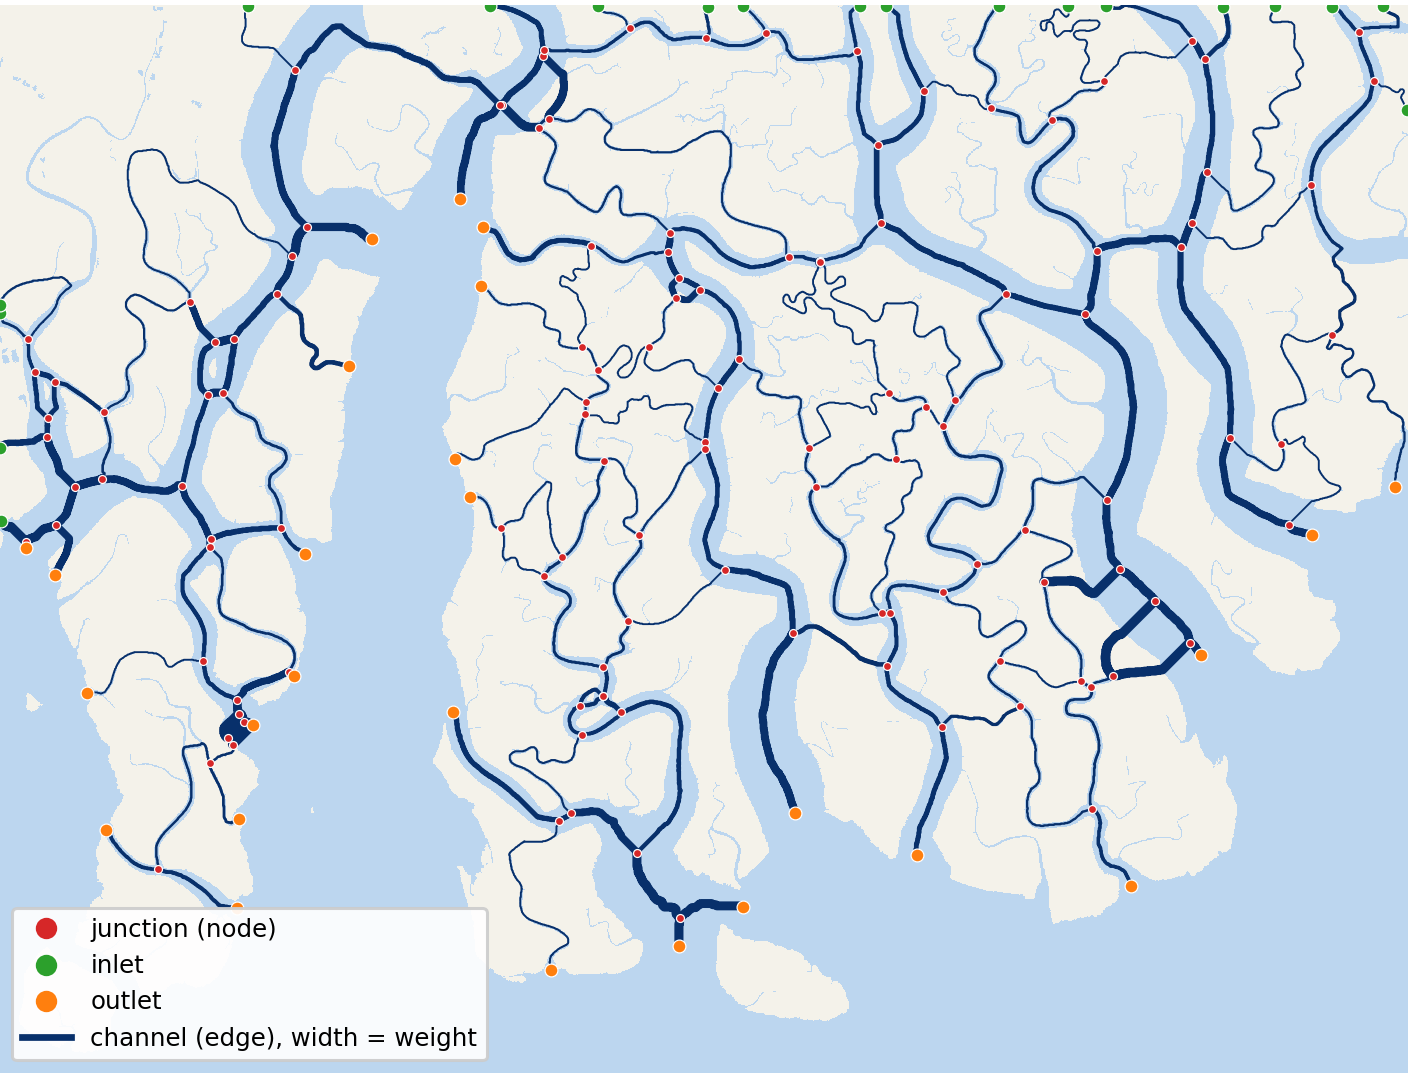
\includegraphics[width=\linewidth]{network_G6.png}

{\scriptsize G6 (2022) on its water mask. Thicker lines are wider channels.\par}
\end{column}
\begin{column}{0.45\textwidth}
\begin{itemize}\setlength{\itemsep}{7pt}
  \item \textbf{What is the network?} Nodes are channel junctions; edges are channels, weighted by width.
  \item \textbf{Planar by definition.} Channels in a 2-D image cannot cross without meeting at a junction.
  \item \textbf{No single flow direction.} Tides push water both ways, so the graph is undirected. A one-way direction only holds for rivers.
  \item \textbf{Not a tree.} The delta has loops: water has several routes between the same two points.
\end{itemize}
\end{column}
\end{columns}
\end{frame}

% ---------------------------------------------------------------- slide 2
\begin{frame}{Properties of the extracted graph}
\begin{columns}[T,onlytextwidth]
\begin{column}{0.42\textwidth}
\small
\begin{enumerate}\setlength{\itemsep}{1pt}
  \item Keep the largest connected component.
  \item Remove degree-0 and degree-1 nodes that are not inlets or outlets.
  \item Remove degree-2 nodes: join their two edges into one.
  \item Split each node of degree $>3$ into degree-3 nodes.
\end{enumerate}

\vspace{1mm}
\begin{block}{What the cleaning preserves}
\small
\begin{itemize}\setlength{\itemsep}{0pt}
  \item Planarity
  \item Loops: $L = E - N + 1$
  \item Node count for a given $L$ (right)
\end{itemize}
\end{block}
\end{column}

\begin{column}{0.56\textwidth}
\centering
\small\textbf{Step 3: remove degree-2 nodes}\\[1mm]
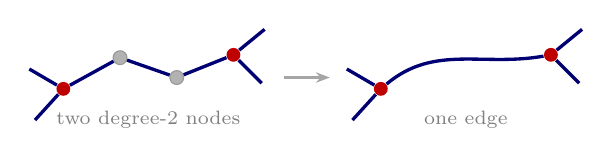
\begin{tikzpicture}[scale=0.72]
  \node[gp-node] (a) at (0,0) {}; \node[gp-deg2] (b) at (1,0.55) {}; \node[gp-deg2] (c) at (2,0.2) {}; \node[gp-node] (d) at (3,0.6) {};
  \draw[gp-chan] (a) -- (b) -- (c) -- (d);
  \draw[gp-chan] (a) -- ++(-0.5,-0.55); \draw[gp-chan] (a) -- ++(-0.6,0.35);
  \draw[gp-chan] (d) -- ++(0.55,0.45); \draw[gp-chan] (d) -- ++(0.5,-0.5);
  \node[font=\scriptsize, gray] at (1.5,-0.55) {two degree-2 nodes};
  \draw[gp-arrow] (3.9,0.2) -- (4.7,0.2);
  \begin{scope}[xshift=5.6cm]
    \node[gp-node] (a2) at (0,0) {}; \node[gp-node] (d2) at (3,0.6) {};
    \draw[gp-chan] (a2) to[out=40, in=190] (d2);
    \draw[gp-chan] (a2) -- ++(-0.5,-0.55); \draw[gp-chan] (a2) -- ++(-0.6,0.35);
    \draw[gp-chan] (d2) -- ++(0.55,0.45); \draw[gp-chan] (d2) -- ++(0.5,-0.5);
    \node[font=\scriptsize, gray] at (1.5,-0.55) {one edge};
  \end{scope}
\end{tikzpicture}

\vspace{2mm}
\textbf{Step 4: split a high-degree node}\\[1mm]
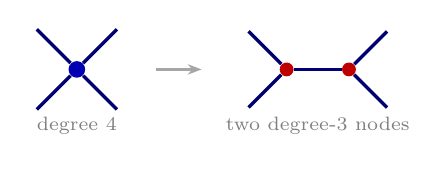
\begin{tikzpicture}[scale=0.72]
  \node[gp-high] (h) at (1.2,0) {};
  \foreach \ang in {45,135,225,315} \draw[gp-chan] (h) -- ++(\ang:1.0);
  \node[font=\scriptsize, gray] at (1.2,-1.0) {degree 4};
  \draw[gp-arrow] (2.6,0) -- (3.4,0);
  \begin{scope}[xshift=4.9cm]
    \node[gp-node] (p) at (0,0) {}; \node[gp-node] (q) at (1.1,0) {};
    \draw[gp-chan] (p) -- (q);
    \draw[gp-chan] (p) -- ++(135:0.95); \draw[gp-chan] (p) -- ++(225:0.95);
    \draw[gp-chan] (q) -- ++(45:0.95); \draw[gp-chan] (q) -- ++(315:0.95);
    \node[font=\scriptsize, gray] at (0.55,-1.0) {two degree-3 nodes};
  \end{scope}
\end{tikzpicture}

{\scriptsize Each step changes $N$ and $E$ by the same amount, so $L$ is unchanged.\par}

\vspace{2mm}
\begin{block}{Node count}
\small
$N = 2(L-1)$ \hfill when every node has degree 3\\[1mm]
$N = 2(L-1) + 2k$ \hfill with $k$ inlet/outlet leaves\\[1mm]
{\scriptsize For example, G1: $142 = 2 \times 34 + 2 \times 37$.}
\end{block}
\end{column}
\end{columns}
\end{frame}

\end{document}
